% !TeX program = pdflatex
% !TeX encoding = UTF-8
%=======================================================================
%  GRIS-NOT-001  ·  Plantilla de notas rápidas para la memoria
%  Proyecto 00503 - Generator inspection robotic system · Mecanalisis
%  Identidad: GRIS-IDENTIDAD-001 v1.4
%-----------------------------------------------------------------------
%  CÓMO USARLA (en 3 pasos)
%
%   1. Copiá este archivo con el código de la nota:
%         memoria/notas/02489-00-MC007.tex
%      El número (###) es correlativo: mirá la última nota y sumá uno.
%
%   2. Completá los cuatro datos del bloque «DATOS DE LA NOTA».
%
%   3. Escribí:
%        · Resultados (obligatorio, siempre primero): lo que se sabe
%          ahora que antes no se sabía. Frases cortas, con números.
%        · El resto es libre. Usá los títulos que te sirvan, o ninguno.
%
%   Compilar:  pdflatex 02489-00-MC007.tex
%   En Overleaf: subí el .tex y logo-gris.pdf.
%
%  LOGO: se usa «logo-gris.pdf» (GRIS-LOGO-003, reducido) de esta carpeta
%  o de ../plantilla/. Si falta, se escribe «GRIS» como marcador.
%=======================================================================
\documentclass[11pt,a4paper]{article}

%=======================================================================
%  DATOS DE LA NOTA  ← lo único que hay que tocar arriba
%=======================================================================
\newcommand{\codigo}{02489-00-MC003}          % 02489-00-MC###
\newcommand{\titulo}{Selección del actuador del paralelogramo}
\newcommand{\autor}{Matías Gaviño}
\newcommand{\fecha}{24/09/2026}                    % o p. ej. {24/09/2026}

%=======================================================================
%  ESTILO  (no hace falta tocar nada de aquí hasta \begin{document})
%=======================================================================
\usepackage[T1]{fontenc}
\usepackage[utf8]{inputenc}
\usepackage[spanish,es-noshorthands,es-tabla]{babel}
\usepackage{lmodern}
\usepackage[a4paper,top=3.0cm,bottom=2.4cm,left=2.4cm,right=2.4cm,
            headheight=20pt,headsep=1.2cm,footskip=1.1cm]{geometry}
\usepackage{microtype}
\usepackage{xcolor}
\usepackage{graphicx}
\usepackage{booktabs}
\usepackage{array}
\usepackage{enumitem}
\usepackage{titlesec}
\usepackage{fancyhdr}
\usepackage{caption}
\usepackage{amsmath,amssymb}
\usepackage{float}
\usepackage[hidelinks]{hyperref}

% --- colores -----------------------------------------------------------
\definecolor{gris-naranja}{HTML}{FF7A00}   % naranja institucional
\definecolor{tinta}{HTML}{1E2328}
\definecolor{gris-medio}{HTML}{6B7280}
\definecolor{gris-linea}{HTML}{DADDE1}
\color{tinta}

\hypersetup{pdftitle={\codigo\ -- \titulo}, pdfauthor={\autor},
            colorlinks=true, linkcolor=tinta, urlcolor=tinta}

% --- logo ---------------------------------------------------------------
\graphicspath{{./}{../plantilla/}{plantilla/}{02489-00-MC003/figuras/}}
\newcommand{\logogris}{%
  \IfFileExists{logo-gris.pdf}
    {
\includegraphics[height=16pt]{logo-gris.pdf}}
    {\IfFileExists{../plantilla/logo-gris.pdf}
      {
\includegraphics[height=16pt]{../plantilla/logo-gris.pdf}}
      {{\fontsize{18}{18}\selectfont\bfseries\sffamily\color{gris-naranja}GRIS}}}}

% --- tipografía del cliente (código documental) --------------------------
% Geogrotesque no es libre; se usa Roboto Condensed Bold, que viene con
% TeX Live y Overleaf y tiene el mismo aire que el logo.
\newcommand{\fuentecliente}{\fontfamily{Roboto-TLF}\fontseries{bc}\selectfont}

% --- encabezado y pie ---------------------------------------------------
\pagestyle{fancy}
\fancyhf{}
\renewcommand{\headrulewidth}{0.4pt}
\renewcommand{\headrule}{\vspace{3pt}{\color{gris-linea}\hrule height \headrulewidth}}
\fancyhead[L]{\logogris}
\fancyhead[R]{{\fuentecliente\fontsize{12}{12}\selectfont\color{gris-medio}\codigo}}
\fancyfoot[R]{\footnotesize\color{gris-medio}\thepage}

% --- títulos numerados ----------------------------------------------------
\setcounter{secnumdepth}{2}
\titleformat{\section}{\large\bfseries}{\thesection}{0.8em}{}
\titleformat{\subsection}{\normalsize\bfseries}{\thesubsection}{0.8em}{}
\titlespacing*{\section}{0pt}{16pt}{5pt}
\titlespacing*{\subsection}{0pt}{11pt}{3pt}

% --- texto ------------------------------------------------------------------
\setlength{\parindent}{0pt}
\setlength{\parskip}{6pt}
\linespread{1.05}
\setlist{topsep=2pt, itemsep=2pt, parsep=0pt, leftmargin=1.2em}
\setlist[itemize]{label={\raisebox{0.15ex}{\small$\bullet$}}}
\captionsetup{font={small,color=gris-medio}, labelfont=bf, skip=5pt}
\renewcommand{\arraystretch}{1.25}

% --- cabecera de la nota ------------------------------------------------------
\newcommand{\cabecera}{%
  \thispagestyle{fancy}%
  {\fontsize{20}{24}\selectfont\bfseries\titulo\par}%
  \vspace{5pt}%
  {\small\color{gris-medio}\fecha\quad·\quad\autor\par}%
  \vspace{6pt}}

% --- ayudas opcionales --------------------------------------------------------
% \figura{archivo}{ancho}{pie}
\newcommand{\figura}[3]{%
  \begin{figure}[htbp]\centering
    \includegraphics[width=#2\linewidth]{#1}\caption{#3}
  \end{figure}}

%=======================================================================
\newcommand{\hoja}[2]{\fbox{\includegraphics[width=#1\linewidth]{#2}}}
\newcommand{\marco}[1]{\fbox{\includegraphics[width=\dimexpr\linewidth-0.6pt\relax]{#1}}}
\setlength{\fboxrule}{0.3pt}\setlength{\fboxsep}{0pt}

\begin{document}
\cabecera

%-----------------------------------------------------------------------
%  RESULTADOS  (siempre primero, lo único obligatorio)
%-----------------------------------------------------------------------
\section{Resultados}
\textbf{Actuador seleccionado: FAULHABER 10L~HL 64:1 con motor paso a paso AM1020}
(AM10202R025008), $\varnothing$10~mm, husillo 3$\times$0,5~mm. Todos los valores salen de las hojas de
datos oficiales (anexo~\ref{sec:anexo}); los cálculos, de \texttt{02489-00-MC003/calculo.py}.

\begin{table}[H]\centering\footnotesize\setlength{\tabcolsep}{4pt}
\begin{tabular}{l l l c}
\toprule
Requisito & Objetivo & 10L HL 64:1 + AM1020 & Cumple\\
\midrule
Ancho máximo           & 12~mm, ideal 10~mm & $\varnothing$10~mm; largo motor + reductora 33,3~mm & sí\\
Fuerza                 & $>$50~N            & 100~N continua; 150~N pico dinámico; 350~N estática & sí ($\times$2)\\
Carrera                & $\approx$8~mm      & husillo de 15 a 100~mm, a pedido & sí\\
Mantener posición      & sí                 & husillo autobloqueante; retención 1,6~mNm con corriente & sí\\
Precisión absoluta     & no crítica         & 100~$\mu$m (husillo estándar); juego de tuerca 80~$\mu$m & sí\\
Velocidad              & secundaria         & 1~mm/s continua: 8~mm en 8~s & sí\\
Robustez               & alta               & carcasa y husillo inoxidables, engranajes de acero & sí\\
Electrónica            & mínima             & paso a paso bipolar en lazo abierto, sin encoder & sí\\
\bottomrule
\end{tabular}
\end{table}

\begin{itemize}
  \item \textbf{Los requisitos crecieron de 15~N a más de 50~N} y la carrera de 5 a 8~mm. Eso descartó la
        primera elección, \textbf{06L~HL + DM0620}: su versión más fuerte (1024:1) da 25~N continuos.
  \item \textbf{El 10L~HL 64:1 da el doble de la fuerza pedida} (100~N) y es el más rápido de la serie.
        Las relaciones 256:1 (150~N) y 1024:1 (200~N) no aportan nada necesario y tardan 27~s y 114~s en
        recorrer 8~mm.
  \item \textbf{El AM1020 tiene margen:} para 100~N necesita 0,51~mNm; a 1~mm/s (7680~min$^{-1}$) entrega
        $\approx$0,88~mNm con una tensión de driver de 2,5 veces la nominal. Para 50~N el margen es de 3,5 veces.
  \item \textbf{El 10L~SL no sirve:} es la versión de carga estándar de la misma serie; con 64:1 da 15~N y
        como máximo 40~N con 1024:1.
  \item \textbf{Descartados:} maxon DCX~10~S + GPX~10 + husillo propio (la reductora admite 5~N axiales:
        habría que diseñar el apoyo axial, la tuerca y el guiado); BLDC (exige inversor trifásico); leva
        excéntrica (par de 0,2~Nm para 50~N, más que los 0,15~Nm continuos del GPX~10, y carga lateral);
        PiezoMotor LEGS (máximo 40~N con 24,2~mm de alto).
  \item \textbf{Pendiente para la integración:} carga radial máxima de \textbf{5~N} sobre el husillo, fuerza
        de choque contra el tope (el motor puede superar los 150~N de pico), referencia de posición sin
        encoder (\emph{homing}) y definición de la tuerca (sección~\ref{sec:riesgos}).
\end{itemize}

%-----------------------------------------------------------------------
\section{Requisitos y cómo cambiaron}
El actuador mueve el módulo a través del paralelogramo y tiene que ser extremadamente compacto. Los
requisitos cambiaron durante la selección:

\begin{table}[H]\centering\small
\begin{tabular}{l l l}
\toprule
Requisito & Etapa inicial & Requisito final\\
\midrule
Diámetro / ancho máximo & $\approx$6~mm (lo más chico posible) & 12~mm, ideal 10~mm\\
Carrera                 & $\approx$5~mm                        & $\approx$8~mm\\
Fuerza                  & $\approx$15~N                        & $>$50~N\\
Uso                     & accionamientos breves                & mantener posición; vida útil prioritaria\\
Precisión absoluta      & no crítica                           & no crítica\\
Velocidad               & --                                   & secundaria\\
Robustez                & --                                   & alta, aplicación industrial\\
Electrónica             & --                                   & lo más compacta posible\\
\bottomrule
\end{tabular}
\end{table}

La carrera corta (8~mm) abrió la puerta a tecnologías distintas del actuador lineal convencional: leva
excéntrica y motores piezoeléctricos. La fuerza de más de 50~N dentro de 10--12~mm fue el requisito que
terminó definiendo la selección.

%-----------------------------------------------------------------------
\section{Primera elección: 06L HL + DM0620}
Con 15~N y 5~mm, la opción fue el FAULHABER \textbf{06L~HL 64:1} con el paso a paso \textbf{DM0620}
(20 pasos por vuelta, 0,25~mNm de retención). Es la misma filosofía que la solución final ---reductora
planetaria y husillo 3$\times$0,5 integrados--- en un tamaño menor: el conjunto mide 24,7~mm de largo.

\begin{table}[H]\centering\small
\caption{Serie 06L~HL (hoja EN\_06L\_HL\_FMO, ed.\ 28/07/2026).}
\begin{tabular}{l c c c}
\toprule
 & 64:1 & 256:1 & 1024:1\\
\midrule
Fuerza axial continua [N]        & 15  & 20  & 25\\
Pico dinámico / estático [N]     & 25 / 80 & 30 / 80 & 35 / 80\\
Velocidad continua [mm/s]        & 1,6 & 0,4 & 0,1\\
Tiempo para 5~mm [s]             & 3,1 & 12,5 & 50\\
\bottomrule
\end{tabular}
\end{table}

Para 15~N el DM0620 necesita 0,076~mNm, muy por debajo de sus 0,25~mNm: era una solución muy atractiva.
\textbf{Al subir el requisito a más de 50~N la familia de 6~mm quedó sin margen}: ni con 1024:1 pasa de
25~N continuos, y su fuerza estática máxima es de 80~N.

%-----------------------------------------------------------------------
\section{Solución elegida: 10L HL 64:1 + AM1020}

\subsection{Datos de la hoja}
La serie 10L~HL (\emph{Gearhead with integrated Lead Screw, high load}) mantiene la arquitectura de la
06L en $\varnothing$10~mm y multiplica la capacidad mecánica.

\begin{table}[H]\centering\small
\caption{Serie 10L~HL (hoja EN\_10L\_HL\_FMO, ed.\ 28/07/2026). En negrita, la relación elegida.}
\label{tab:10lhl}
\begin{tabular}{l c c c}
\toprule
 & \textbf{64:1} & 256:1 & 1024:1\\
\midrule
Fuerza axial continua [N]                 & \textbf{100} & 150 & 200\\
Pico dinámico [N]                         & \textbf{150} & 200 & 250\\
Pico estático [N]                         & \textbf{350} & 350 & 350\\
Velocidad continua / pico [mm/s]          & \textbf{1 / 2,1} & 0,3 / 0,5 & 0,07 / 0,1\\
Entrada cont.\ / pico [min$^{-1}$] & \multicolumn{3}{c}{8000 / 16\,000}\\
$\eta$ reductora / husillo, máx. [\%] & \textbf{70 / 35} & 60 / 35 & 55 / 35\\
Largo L2 / con AM1020 L1 [mm]   & \textbf{17,4 / 33,3} & 20,5 / 36,4 & 23,6 / 39,5\\
Masa [g]                                  & \textbf{10,1} & 11,2 & 13,3\\
Tiempo 8~mm, cont.\ / pico [s]     & \textbf{8 / 3,8} & 27 / 16 & 114 / 80\\
\midrule
Husillo & \multicolumn{3}{l}{3$\times$0,5~mm, perfil de rosca propio; acero inoxidable}\\
Tuerca estándar & \multicolumn{3}{l}{cilíndrica, plástica; juego axial 80~$\mu$m}\\
Carcasa / engranajes / cojinetes & \multicolumn{3}{l}{acero inoxidable / acero / rodamientos de bolas precargados}\\
Carga radial máx. (50~mm de la brida) & \multicolumn{3}{l}{5~N}\\
Pandeo del husillo estándar & \multicolumn{3}{l}{195~N (empotrado--libre); 1563~N (empotrado--apoyado)}\\
Temperatura de operación & \multicolumn{3}{l}{$-30$ a $+80$~°C}\\
\bottomrule
\end{tabular}
\end{table}

\begin{figure}[H]\centering
  \hoja{0.48}{ds_10L_HL_p1.png}\hfill\hoja{0.48}{ds_10L_HL_p2.png}
  \caption{Hoja de datos FAULHABER 10L~HL: datos técnicos, zonas de operación recomendadas, plano y
  combinaciones con motores (AM1020...08: L1 = 33,3~mm con 64:1).}
\end{figure}

\subsection{Relación de reducción}
El 64:1 ya duplica la fuerza pedida y es el único que recorre los 8~mm en segundos. El 256:1 y el 1024:1
suben la fuerza continua a 150 y 200~N, que no se necesitan, y alargan la carrera a 27~s y 114~s.

\subsection{Motor AM1020 y punto de operación}
El AM1020 es un paso a paso de dos fases, 20 pasos por vuelta, $\varnothing$10$\times$15,9~mm y 5,5~g.
La variante del CAD (\texttt{AM10202R025008}) es la de rodamientos de bolas precargados (2R), bobinado
0250 (2~V, 0,25~A por fase, 8~$\Omega$) y piñón para reductoras 10/1 (opción 08), que es la que se acopla
al 10L.

El par de motor necesario para una fuerza $F$ en la tuerca es
\begin{equation}
T_m=\frac{F\,p}{2\pi\,\eta_s\,\eta_g\,i},
\end{equation}
con $p=0{,}5$~mm, $i=64$ y los rendimientos máximos de la hoja ($\eta_s=0{,}35$, $\eta_g=0{,}70$). Da
\textbf{0,25~mNm para 50~N y 0,51~mNm para 100~N}. Como los rendimientos son máximos, el par real es algo
mayor. La velocidad de motor es $n_m=60\,v\,i/p$: 1~mm/s pide 7680~min$^{-1}$ y 2,1~mm/s, 16\,128~min$^{-1}$.

\begin{figure}[H]\centering
  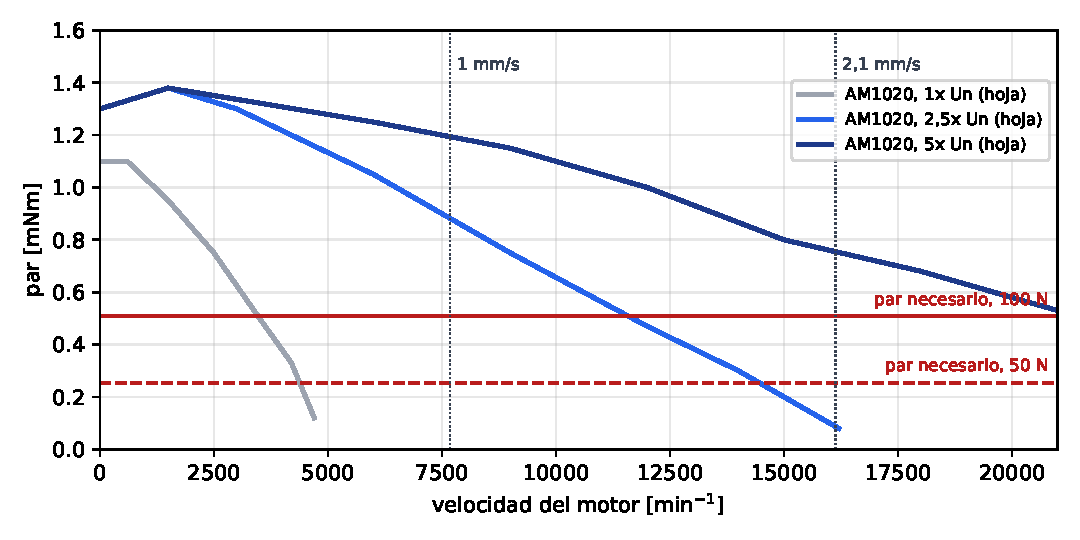
\includegraphics[width=0.85\linewidth]{fig_par_am1020.pdf}
  \caption{Curvas par--velocidad del AM1020 (digitalizadas de la hoja, $\pm$0,05~mNm) frente al par
  necesario con el 10L~HL 64:1. «2,5x Un»: driver chopper con 2,5 veces la tensión nominal y corriente
  limitada a la nominal.}
  \label{fig:par}
\end{figure}

\begin{itemize}
  \item \textbf{A 1~mm/s} el motor entrega $\approx$0,88~mNm (2,5$\times$U$_n$) o $\approx$1,19~mNm
        (5$\times$U$_n$): margen de 1,7 a 2,3 veces sobre 100~N, y de 3,5 a 4,7 veces sobre 50~N.
  \item \textbf{A 2,1~mm/s} hace falta 5$\times$U$_n$ ($\approx$0,75~mNm disponibles) y se está en el
        límite de 16\,000~min$^{-1}$ de entrada de la reductora: sirve para maniobras cortas, no como régimen.
  \item \textbf{Con 1$\times$U$_n$} (sin driver chopper) el motor solo llega a $\approx$3500~min$^{-1}$ con 0,5~mNm:
        $\approx$0,45~mm/s y 18~s para 8~mm.
\end{itemize}

\begin{figure}[H]\centering
  \hoja{0.48}{ds_AM1020_p1.png}\hfill
  \begin{minipage}[b]{0.49\linewidth}\centering
    \marco{ds_AM1020_curva.png}\\[4pt]
    {\small\color{gris-medio}Detalle de la curva de la hoja.}
  \end{minipage}
  \caption{Hoja de datos FAULHABER AM1020 (ed.\ 28/07/2026).}
\end{figure}

\subsection{HL frente a SL}
Las dos variantes de la serie 10L son \emph{gearhead with integrated lead screw}: ambas tienen reductora
planetaria y el mismo husillo 3$\times$0,5. La diferencia es la \textbf{capacidad de carga}: SL es la
versión estándar (\emph{standard load}) y HL la de carga alta (\emph{high load}).

\begin{table}[H]\centering\small
\caption{10L~SL frente a 10L~HL (hojas EN\_10L\_SL\_FMO y EN\_10L\_HL\_FMO).}
\begin{tabular}{l c c}
\toprule
 & 10L SL & 10L HL\\
\midrule
Fuerza continua con 64:1 [N]      & 15 & 100\\
Fuerza continua máxima [N]        & 40 (1024:1) & 200 (1024:1)\\
Pico estático [N]                 & 60 & 350\\
Largo sin motor, 64:1 [mm]        & 16,9 & 17,4\\
\bottomrule
\end{tabular}
\end{table}

Con 0,5~mm más de largo, el HL multiplica por 6,7 la fuerza continua con 64:1. El SL no llega a 50~N en
ninguna relación.

\subsection{Husillo, tuerca y roscas}
\begin{itemize}
  \item \textbf{El husillo no es una M3$\times$0,5:} la hoja lo define como «3x0,5 (mm) proprietary thread
        profile». Para fabricar una tuerca propia (p.\ ej.\ con RapidDirect) hay que obtener antes de
        FAULHABER el perfil, las tolerancias y el material recomendado.
  \item \textbf{Tuercas de FAULHABER:} cilíndrica plástica (estándar), cilíndrica de bronce (KWN1), con
        brida de bronce (KWN3), con brida plástica (KWN4) o sin tuerca (KWN9).
  \item \textbf{La M7$\times$0,5-6g} del plano es la rosca de montaje de la brida frontal de la reductora, no la
        de transmisión.
  \item \textbf{Largo del husillo:} 49~mm estándar; de 15 a 100~mm en pasos de 1~mm (opciones KL). La carrera
        útil es el largo roscado menos el largo de la tuerca.
  \item \textbf{Mantener posición:} FAULHABER declara autobloqueantes sus husillos de rosca (figura~\ref{fig:ti}),
        coherente con un rendimiento del husillo menor al 50\,\%. Sin corriente, la carga no debería hacer
        retroceder el conjunto; con corriente, el AM1020 retiene con 1,6~mNm. \textbf{Verificar en ensayo.}
\end{itemize}

\begin{figure}[H]\centering
  \begin{minipage}[b]{0.62\linewidth}\centering
    \marco{ti_estructura.png}
  \end{minipage}\hfill
  \begin{minipage}[b]{0.35\linewidth}\centering
    \marco{ti_selflocking.png}
  \end{minipage}
  \caption{FAULHABER, \emph{Geared Linear Actuators -- Technical Information}. Izquierda: estructura
  interna (brida de motor, reductora planetaria, eje de salida, rodamientos, brida frontal y husillo
  con tuerca). Derecha: comparación husillo de rosca / husillo de bolas; \emph{self-locking}: sí.}
  \label{fig:ti}
\end{figure}

La estructura muestra por qué se eligió: \textbf{la cadena motor $\rightarrow$ reductora $\rightarrow$
apoyo de salida $\rightarrow$ husillo $\rightarrow$ tuerca viene resuelta en $\varnothing$10~mm}, con los
rodamientos que toman la carga axial.

%-----------------------------------------------------------------------
\section{Alternativas descartadas}

\begin{figure}[H]\centering
  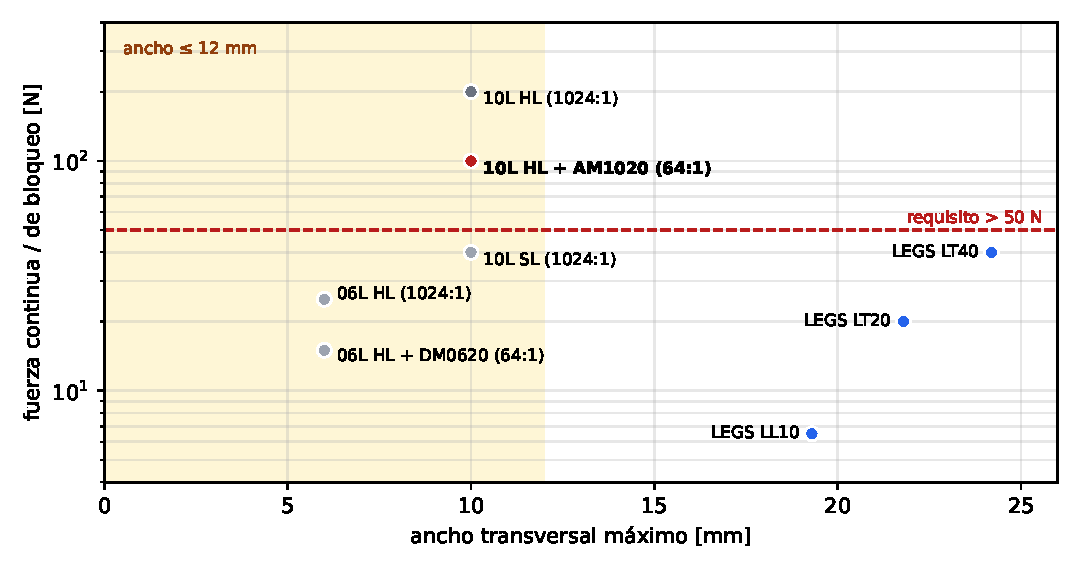
\includegraphics[width=0.85\linewidth]{fig_mapa_candidatos.pdf}
  \caption{Fuerza continua (FAULHABER) o de bloqueo (PiezoMotor) frente al ancho transversal máximo, según
  las hojas de datos. Solo el 10L~HL cae en la zona de $\le$12~mm y $>$50~N.}
  \label{fig:mapa}
\end{figure}

\subsection{maxon DCX 10 S + GPX 10 + husillo externo}
La idea era separar motor + reductora comerciales + husillo comprado + tuerca propia. El motor no es el
problema: el DCX~10~S tiene 0,9~mNm nominales a 14\,300~min$^{-1}$, y el GPX~10 de 3 etapas (64:1)
transmite 0,10~Nm continuos, suficiente en teoría para $\approx$440~N con un husillo 3$\times$0,5.

\textbf{El problema es la carga axial: el GPX~10 admite 5~N} (dinámica, todas las etapas). Para empujar
más de 50~N hay que agregar dentro de 10--12~mm un acople, un rodamiento axial, el husillo, la tuerca y
el guiado, que el 10L~HL ya trae resueltos. El GP~8~S es demasiado chico para la fuerza y el GP~16~S
excede el diámetro objetivo. Además, un motor de corriente continua necesita encoder (ENX~10) para
posicionar.

\begin{figure}[H]\centering
  \hoja{0.48}{ds_GPX10.png}\hfill\hoja{0.48}{ds_DCX10S.png}
  \caption{Hojas maxon (catálogo 2025, páginas 373 y 99): GPX~10 (\emph{Max.\ axial load (dynamic)}: 5~N)
  y DCX~10~S.}
\end{figure}

\subsection{Motores sin escobillas (BLDC)}
Tanto FAULHABER como maxon ofrecen BLDC de $\varnothing$10~mm compatibles: densidad de potencia, vida útil,
suavidad y control por FOC. La penalización es la \textbf{electrónica}: inversor trifásico y conmutación,
en un volumen que no tenemos, para mover 8~mm despacio. En la tabla de combinaciones del 10L~HL, además, el
BLDC 1028...B deja el conjunto en 45,5~mm frente a 33,3~mm con el AM1020. Queda como opción técnicamente
buena pero peor para esta arquitectura.

\subsection{Leva excéntrica}
Con excentricidad $e=4$~mm la carrera es $S=2e=8$~mm. Sin rozamiento, el par en el eje es
$T=F\,e\sin\theta$, máximo a 90°: \textbf{0,2~Nm para 50~N}, más que los 0,15~Nm continuos del GPX~10 más
grande. A eso se suman la carga lateral, la ventaja mecánica muy variable con el ángulo, el seguidor con
rodamientos, más piezas, volumen transversal y una integración peor con el paralelogramo. No simplifica
el mecanismo frente al 10L~HL.

\subsection{PiezoMotor LEGS}
Es la alternativa tecnológica más interesante: movimiento lineal directo, sin juego, y \textbf{retención
sin consumo} (\emph{no power draw in hold position}). El límite vuelve a ser fuerza frente a tamaño:

\begin{table}[H]\centering\small
\caption{PiezoMotor LEGS (hojas LL10AD-2608, LT20ACD-2608, LT40-2608).}
\begin{tabular}{l c c c c}
\toprule
Modelo & Fuerza de bloqueo [N] & L$\times$H$\times$D [mm] & Masa [g] & Driver\\
\midrule
LL10 & 6,5 & 22$\times$19,3$\times$10,8 & 23 & PMD301/401, 48~V\\
LT20 & 20  & 22$\times$21,8$\times$10,8 & 29 & PMD301/401, 48~V\\
LT40 & 40  & 32,1$\times$24,2$\times$23,1 & 61 & PMD301/401, 48~V\\
\bottomrule
\end{tabular}
\end{table}

Ninguno llega a 50~N y el más fuerte mide 24,2~mm de alto. Tampoco da, ante golpes o caídas, la
tranquilidad de un conjunto de acero con reductora y husillo. Queda como tecnología interesante, no como
primera elección.

\begin{figure}[H]\centering
  \hoja{0.48}{ds_LT20_p1.png}\hfill\hoja{0.48}{ds_LT20_p2.png}
  \caption{Hoja PiezoMotor LT20ACD: 20~N de bloqueo en 22$\times$21,8$\times$10,8~mm.}
\end{figure}

%-----------------------------------------------------------------------
\section{Riesgos de integración y pendientes}
\label{sec:riesgos}
\begin{itemize}
  \item \textbf{Carga radial:} el husillo admite 5~N radiales a 50~mm de la brida. La unión con el
        paralelogramo tiene que llevar articulación o guiado de la tuerca para no cargarlo lateralmente.
  \item \textbf{Choque contra tope:} con 1,6~mNm y los rendimientos máximos, el motor podría empujar hasta
        $\approx$315~N, por encima de los 150~N de pico dinámico. Limitar la corriente del driver o prever
        topes que no bloqueen el husillo.
  \item \textbf{Referencia de posición:} en lazo abierto no hay encoder. Hace falta \emph{homing} (fin de
        carrera o detección de pérdida de paso) al arrancar.
  \item \textbf{Driver:} bipolar de dos fases en modo chopper, con 2,5 a 5 veces la tensión nominal
        (5 a 10~V para el bobinado de 2~V) y corriente limitada a 0,25~A.
  \item \textbf{Tuerca propia:} pedir a FAULHABER el perfil del husillo antes de fabricarla.
  \item \textbf{Vida útil:} FAULHABER no da una vida fija; depende de tuerca, carga, velocidad, temperatura y
        ciclo de trabajo. Consultar con el ciclo real.
  \item \textbf{Integración geométrica:} verificada con el CAD del conjunto
        (\texttt{FAULHABER\_10L\_HL\_64\_1\_\allowbreak AM10202R025008\_\allowbreak conjunto.stp}),
        que no está versionado en este repositorio.
\end{itemize}

%-----------------------------------------------------------------------
\section{Anexo: hojas de datos}
\label{sec:anexo}
Las hojas completas están en \texttt{02489-00-MC003/fuentes/}. Direcciones de descarga (septiembre 2026):

{\small
\begin{itemize}
  \item FAULHABER 10L~HL, 10L~SL, 06L~HL y \emph{Technical Information}: \url{https://eshop.faulhaber.com}
        (páginas de las series 10L...HL, 10L...SL, 06L...HL).
  \item FAULHABER AM1020 y DM0620 (EN\_AM1020\_FPS.pdf y EN\_DM0620\_FPS.pdf):\newline
        \url{https://www.faulhaber.com/fileadmin/Import/Media/}.
  \item maxon GPX~10 y DCX~10~S: catálogo maxon 2025, páginas 373 y 99 (\url{https://www.maxongroup.com}).
  \item PiezoMotor LL10, LT20, LT40: \url{https://piezomotor.com}.
\end{itemize}}

\begin{figure}[H]\centering
  \hoja{0.48}{ds_06L_HL_p1.png}\hfill\hoja{0.48}{ds_DM0620_p1.png}
  \caption{FAULHABER 06L~HL y DM0620: la primera elección.}
\end{figure}

\begin{figure}[H]\centering
  \hoja{0.48}{ds_10L_SL_p1.png}\hfill\hoja{0.48}{ds_LT40_p2.png}
  \caption{FAULHABER 10L~SL (carga estándar) y PiezoMotor LT40 (40~N).}
\end{figure}

\end{document}
